\subsection{Results}\label{sec:m1:results}

\subsubsection{Tests}\label{sec:m1:results:tests}

\begin{figure}
    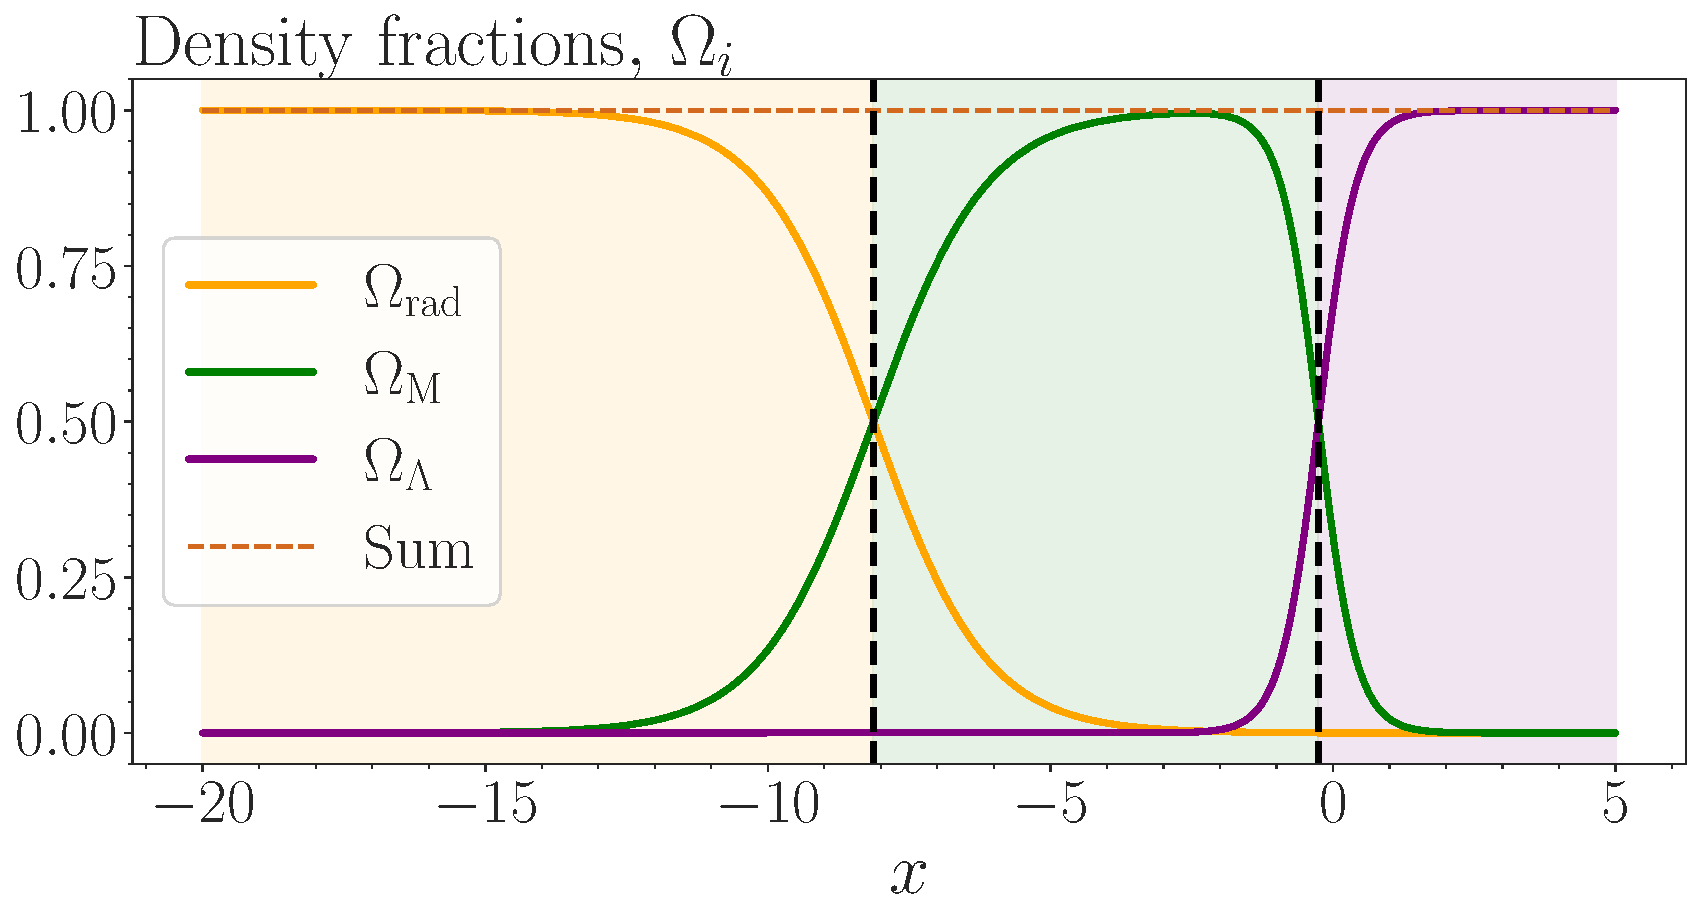
\includegraphics[width=\linewidth]{testing_omegas.pdf}
    \caption{Density fractions $\O_i$ as function of $x$. For low $x$, radiation dominates, before matter dominates and dark has just become the dominant energy density today $x=0$, and will continue to dominate into the future. The sum of densities sums to one across all times, as required.}
    \label{fig:m1:omega_tests}
\end{figure}

\begin{figure}
    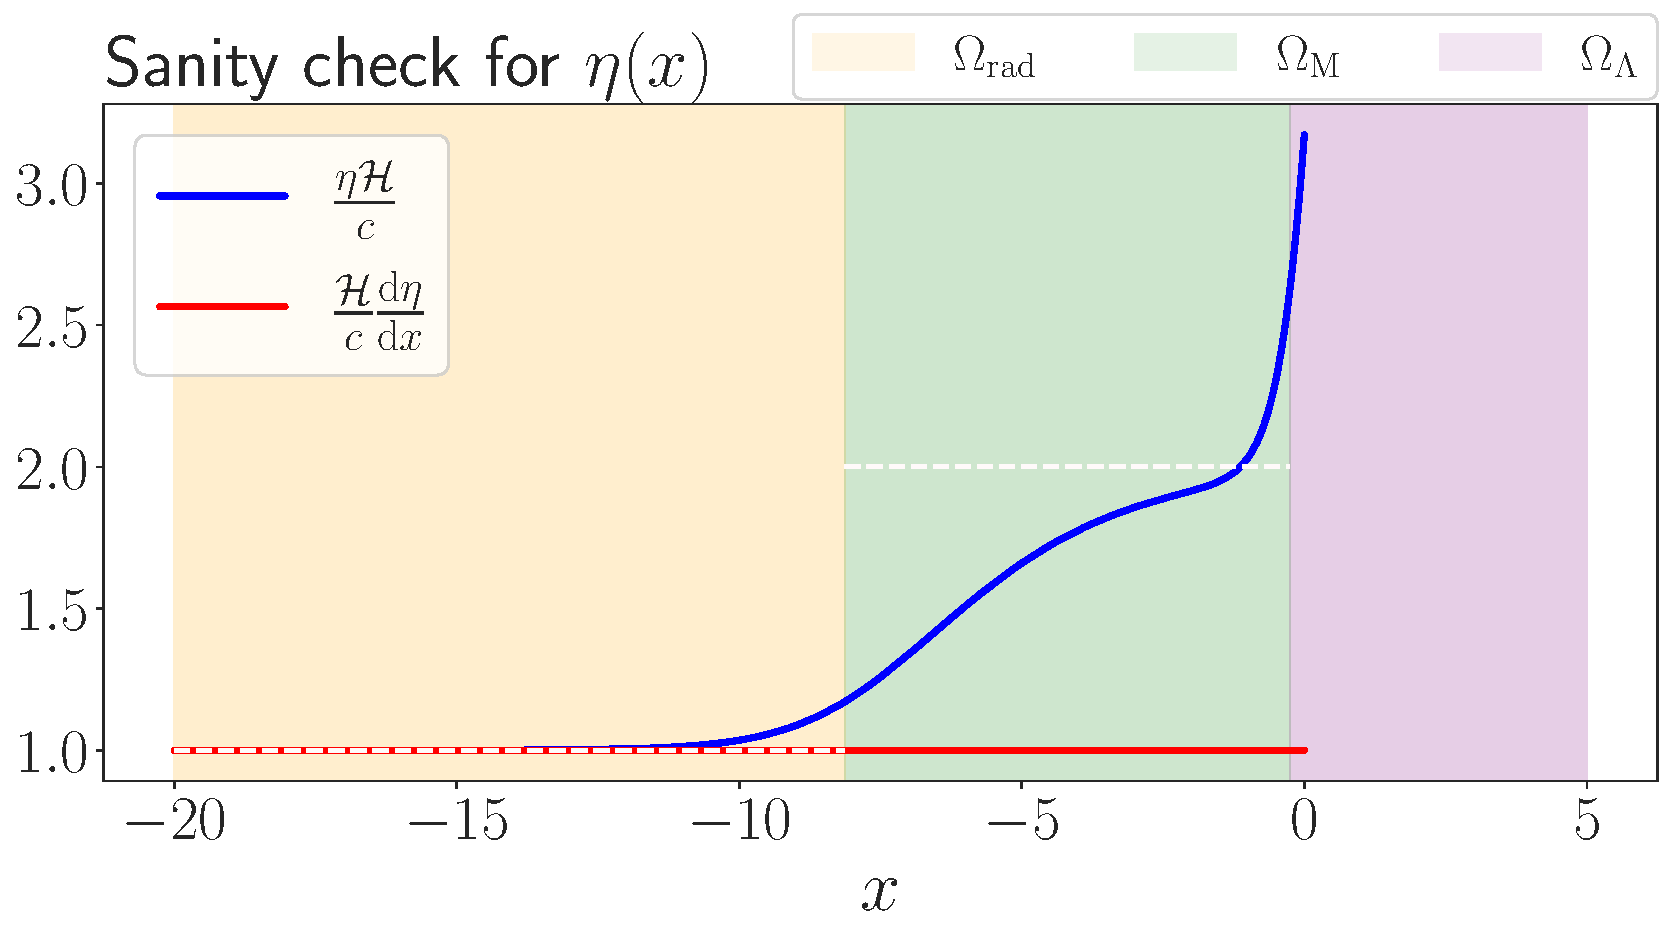
\includegraphics[width=\linewidth]{eta_test.pdf}
    \caption{Eta tests}
    \label{fig:m1:eta_tests}
\end{figure}

\begin{figure}
    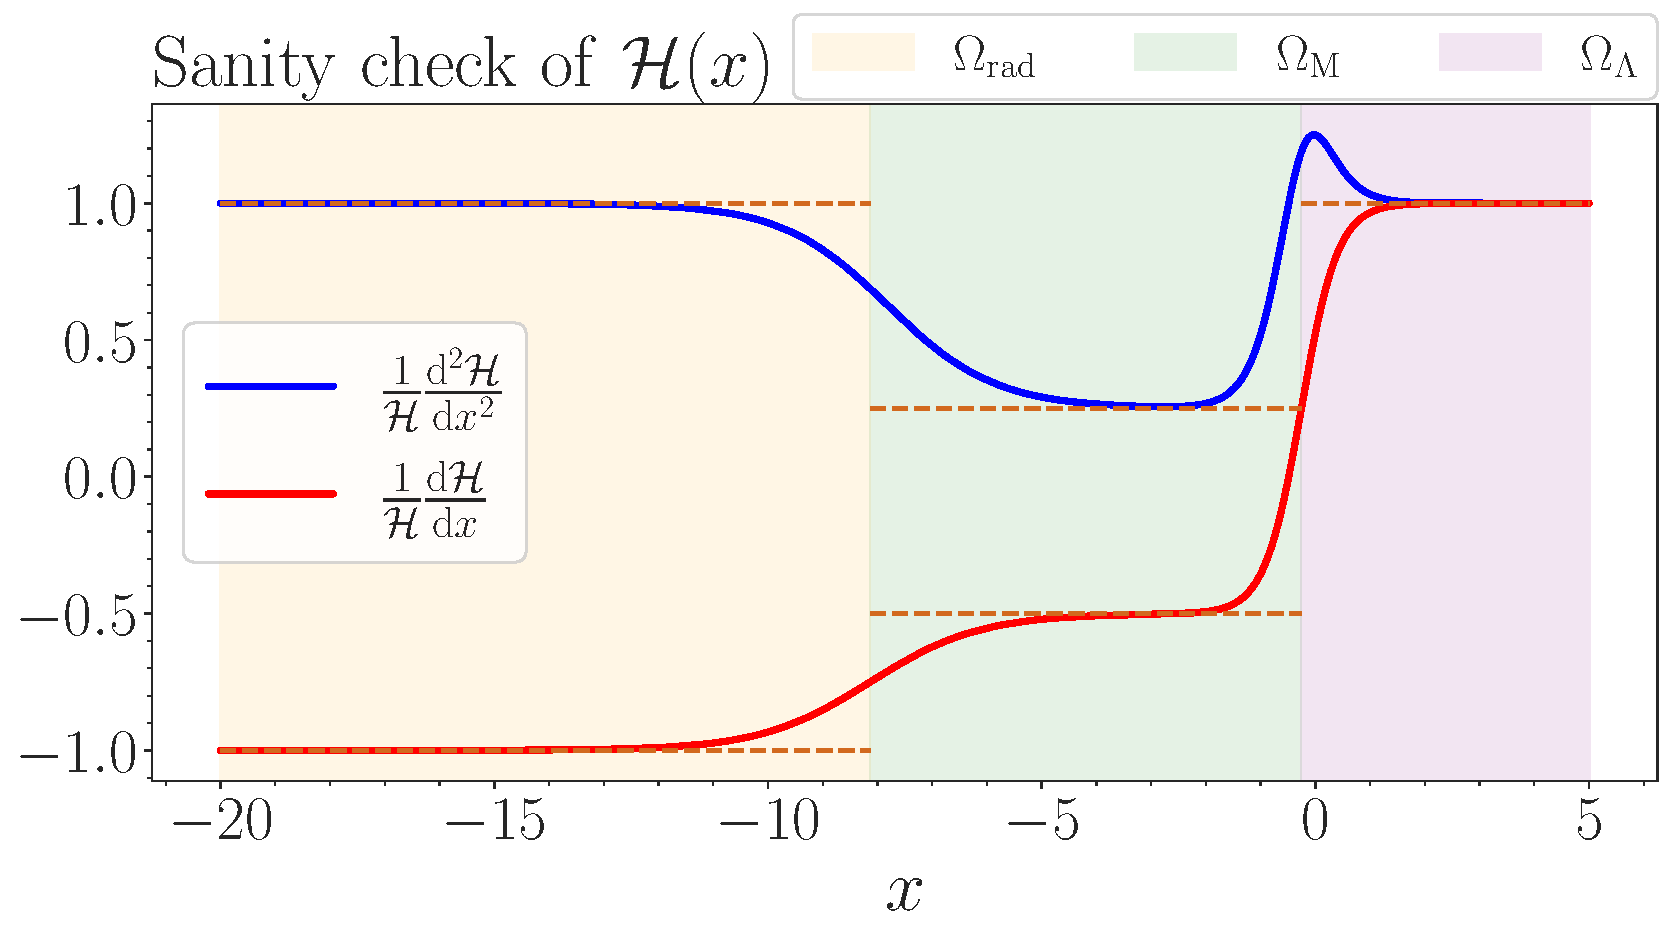
\includegraphics[width=\linewidth]{Hp_test.pdf}
    \caption{HP tests}
    \label{fig:m1:Hp_tests}
\end{figure}

\subsubsection{Analysis}

\begin{tabular}{lrrrl}
Quantity & x & z & t [Gyr] &  \\
RM-equality  & -8.13 & 3400.33 & 0.000051 &   \\
ML-equality  & -0.26 & 0.29 & 10.378200 &   \\
Accel. start  & -0.26 & 0.29 & 10.378200 &    \\
Age of universe  & 0.00 & 0.00 & 13.857700 &   \\
Conformal time  & 0.00 & 0.00 & 46.318700 &   \\
\end{tabular}


\begin{figure}
    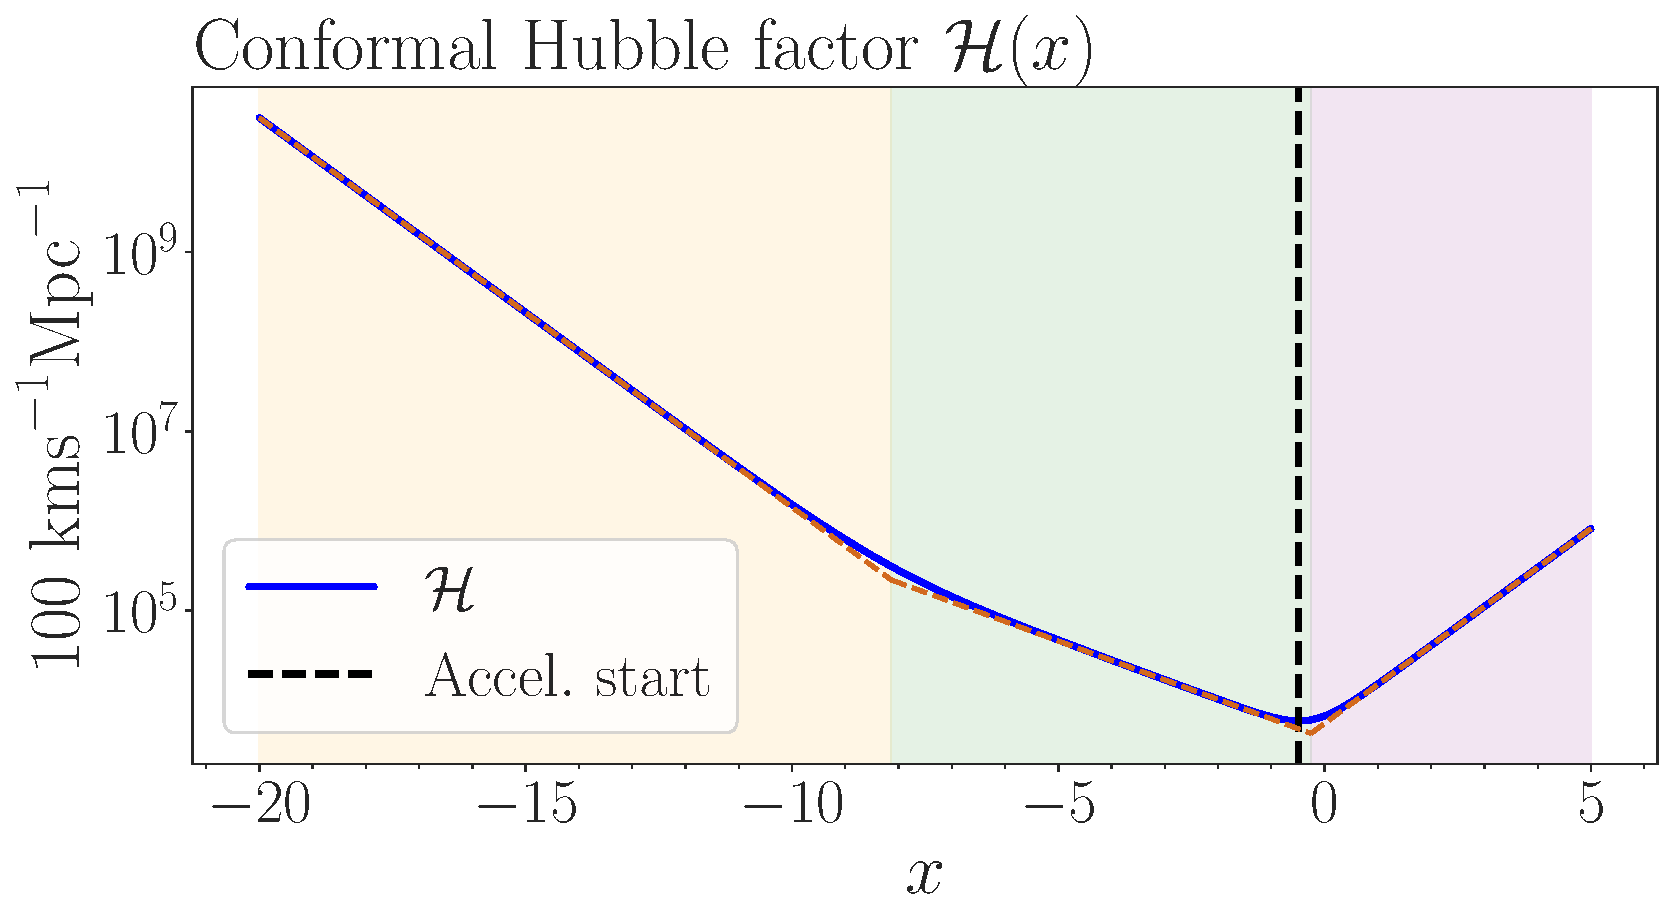
\includegraphics[width=\linewidth]{conformal_hubble_factor.pdf}
    \caption{Conformal Hubble factor.}
    \label{fig:m1:conformal_hubble_factor_Hp}
\end{figure}

\begin{figure}
    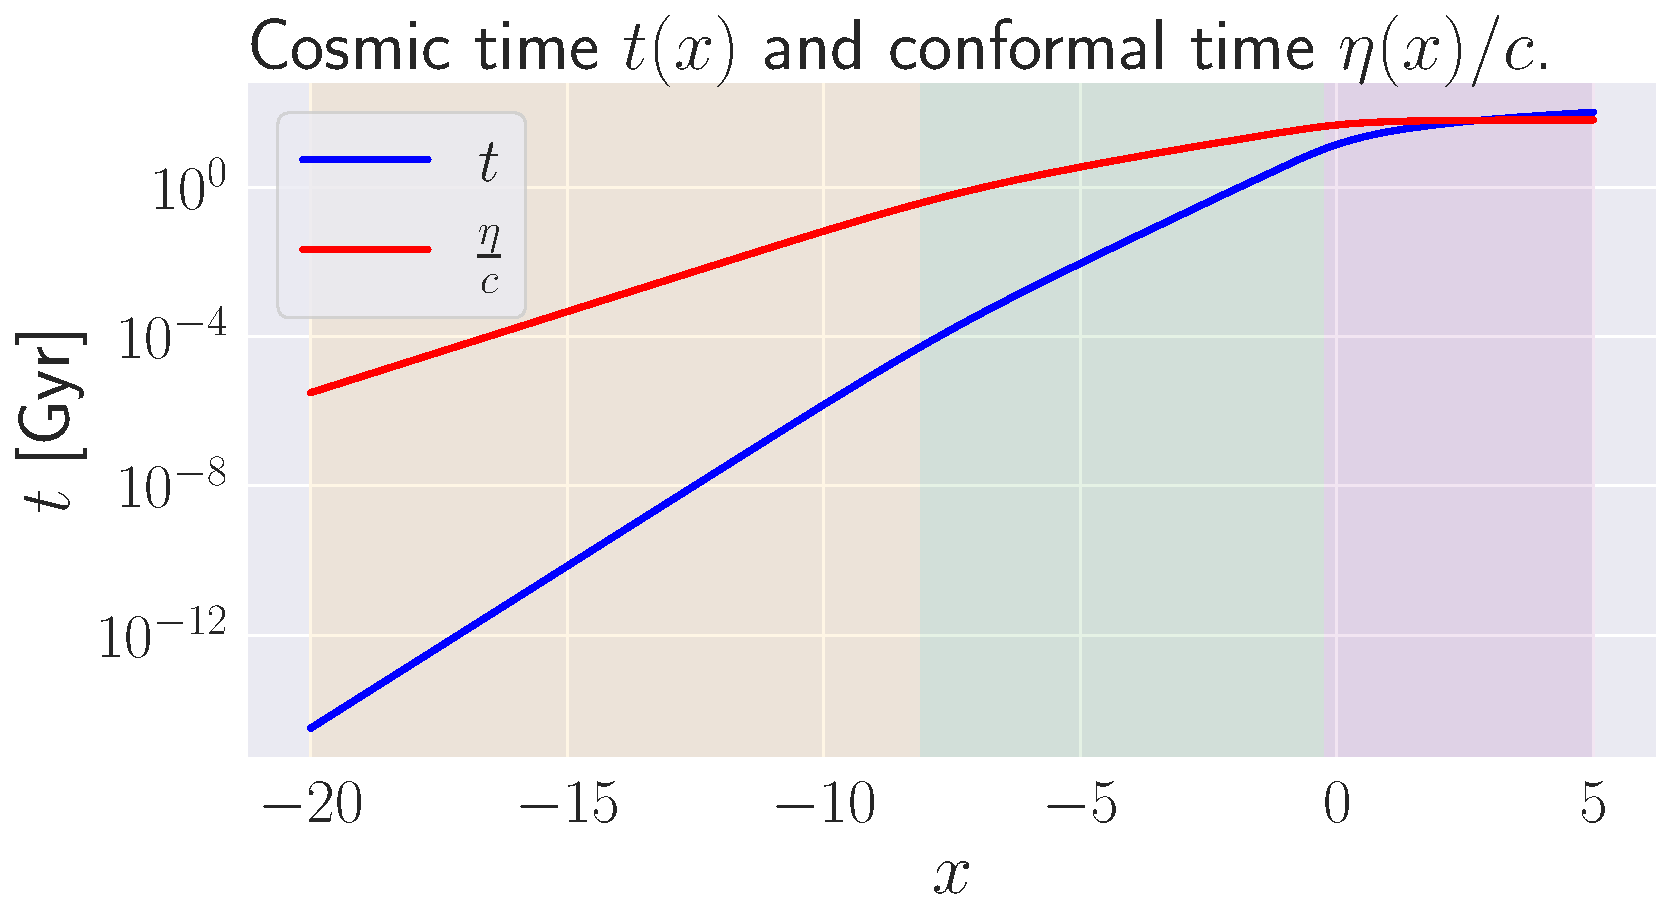
\includegraphics[width=\linewidth]{cosmic_conformal_time.pdf}
    \caption{cosmic time.}
    \label{fig:m1:cosmic_conformal_time}
\end{figure}

\begin{figure}
    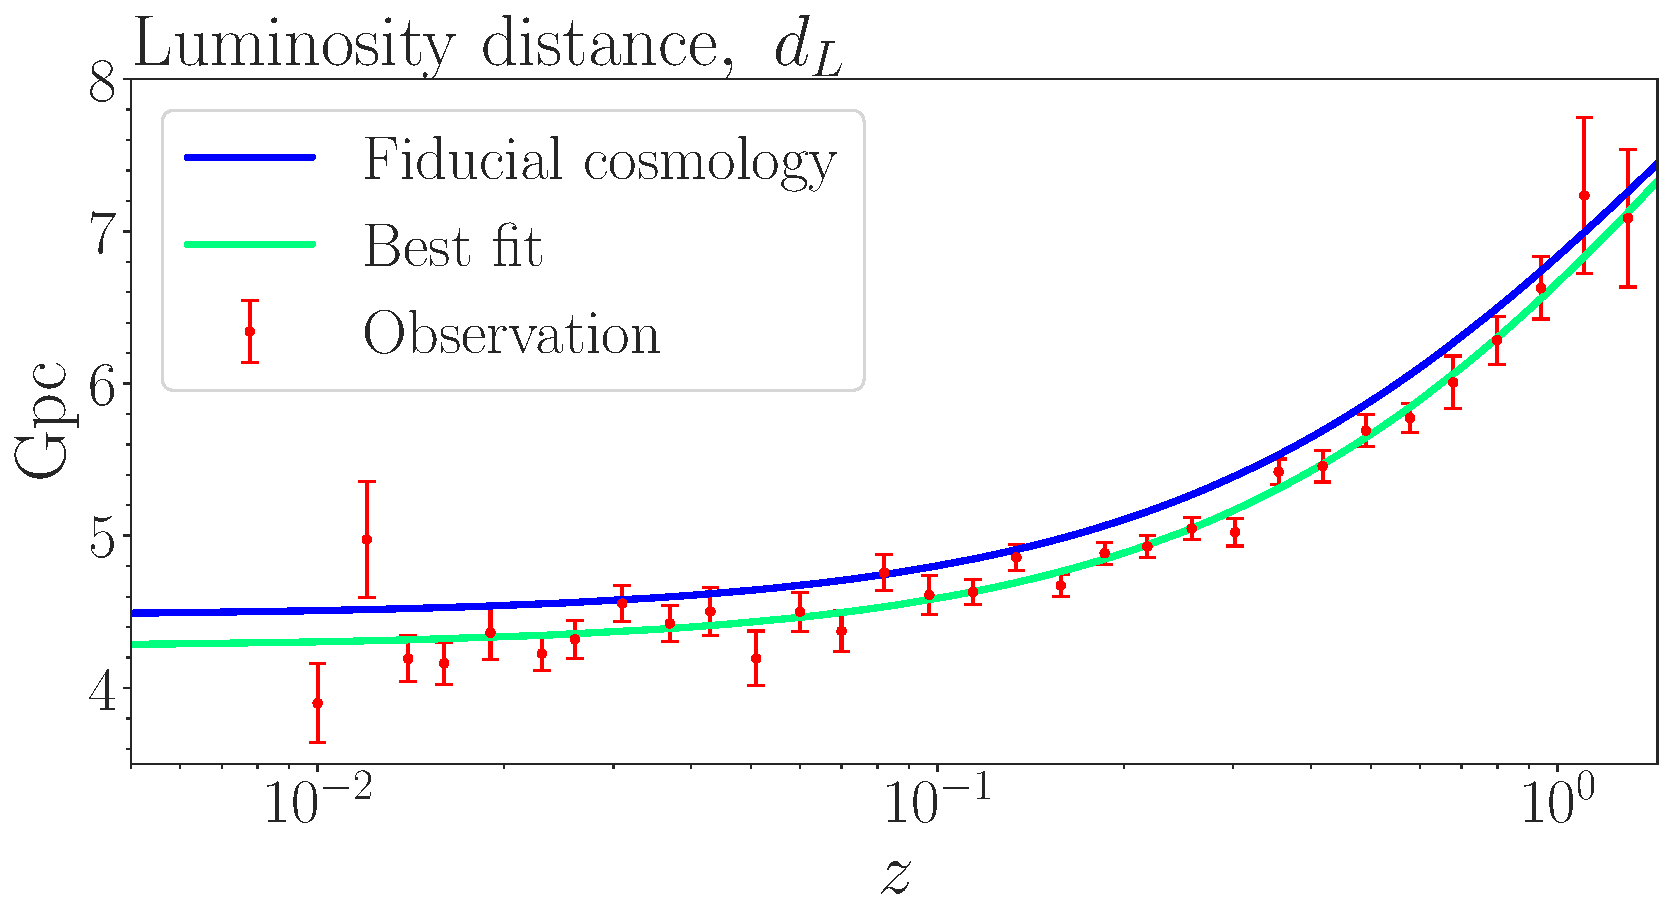
\includegraphics[width=\linewidth]{supernova_data.pdf}
    \caption{Supernova data fitted}
    \label{fig:m1:supernova_data}
\end{figure}

\begin{figure}
    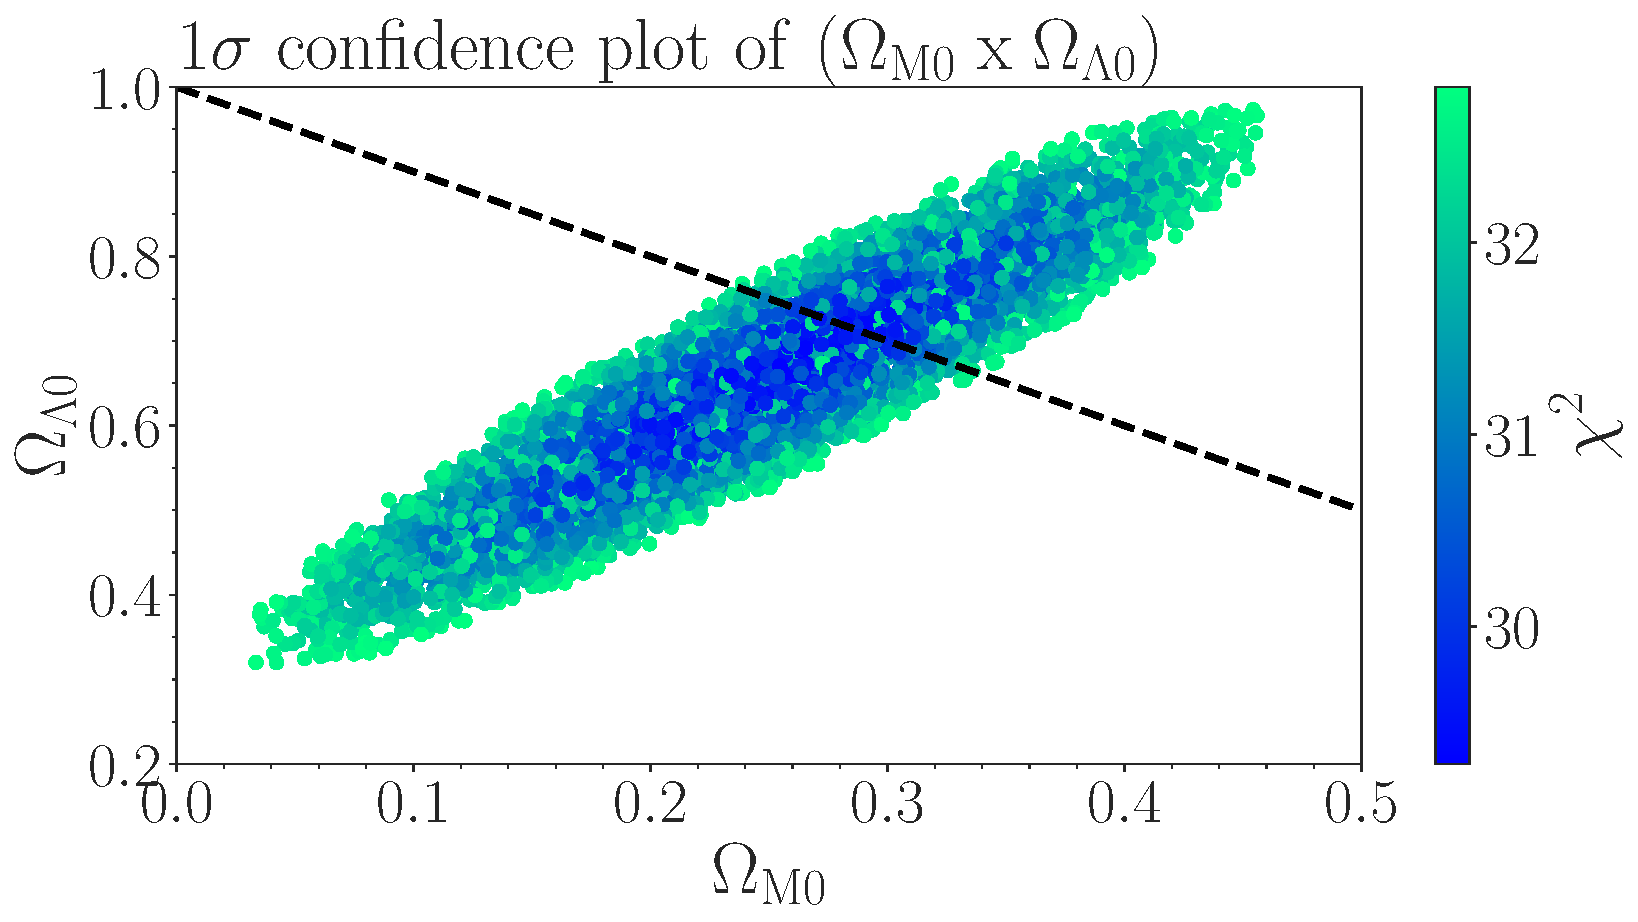
\includegraphics[width=\linewidth]{omega_plane.pdf}
    \caption{one sigma confidence plot}
    \label{fig:m1:omega_planes}
\end{figure}

\begin{figure}
    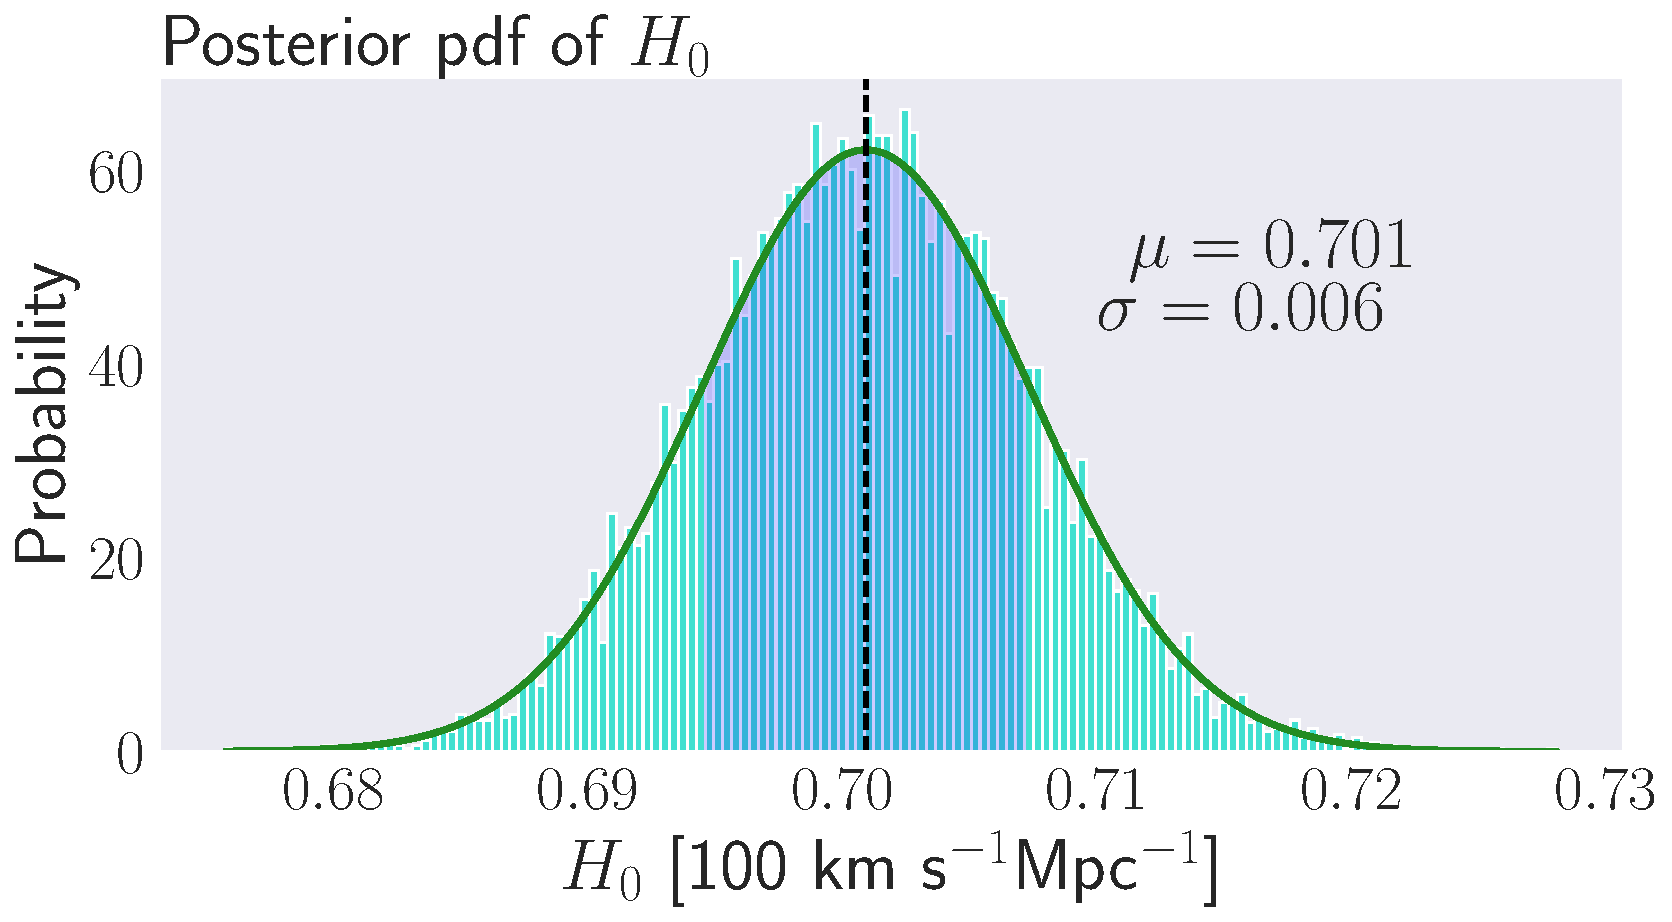
\includegraphics[width=\linewidth]{posterior_pdf.pdf}
    \caption{posterior pdf.}
    \label{fig:m1:posterior_pdf}
\end{figure}

